%%%%%%%%%%%%%%%%%%%%%%%%%%%%%%%%%%%%%%%%%
% Short Sectioned Assignment
% LaTeX Template
% Version 1.0 (5/5/12)
%
% This template has been downloaded from:
% http://www.LaTeXTemplates.com
%
% Original author:
% Frits Wenneker (http://www.howtotex.com)
%
% License:
% CC BY-NC-SA 3.0 (http://creativecommons.org/licenses/by-nc-sa/3.0/)
%
%%%%%%%%%%%%%%%%%%%%%%%%%%%%%%%%%%%%%%%%%

%----------------------------------------------------------------------------------------
%	PACKAGES AND OTHER DOCUMENT CONFIGURATIONS
%----------------------------------------------------------------------------------------

\documentclass[paper=a4, fontsize=11pt]{scrartcl} % A4 paper and 11pt font size

\usepackage[T1]{fontenc} % Use 8-bit encoding that has 256 glyphs
\usepackage{fourier} % Use the Adobe Utopia font for the document - comment this line to return to the LaTeX default
\usepackage[english]{babel} % English language/hyphenation
\usepackage{amsmath,amsfonts,amsthm} % Math packages

\usepackage{lipsum} % Used for inserting dummy 'Lorem ipsum' text into the template

\usepackage{sectsty} % Allows customizing section commands
\allsectionsfont{\centering \normalfont\scshape} % Make all sections centered, the default font and small caps

\usepackage{fancyhdr} % Custom headers and footers
\pagestyle{fancyplain} % Makes all pages in the document conform to the custom headers and footers
\fancyhead{} % No page header - if you want one, create it in the same way as the footers below
\fancyfoot[L]{} % Empty left footer
\fancyfoot[C]{} % Empty center footer
\fancyfoot[R]{\thepage} % Page numbering for right footer
\renewcommand{\headrulewidth}{0pt} % Remove header underlines
\renewcommand{\footrulewidth}{0pt} % Remove footer underlines
\setlength{\headheight}{13.6pt} % Customize the height of the header

\numberwithin{equation}{section} % Number equations within sections (i.e. 1.1, 1.2, 2.1, 2.2 instead of 1, 2, 3, 4)
\numberwithin{figure}{section} % Number figures within sections (i.e. 1.1, 1.2, 2.1, 2.2 instead of 1, 2, 3, 4)
\numberwithin{table}{section} % Number tables within sections (i.e. 1.1, 1.2, 2.1, 2.2 instead of 1, 2, 3, 4)

%\setlength\parindent{0pt} % Removes all indentation from paragraphs - comment this line for an assignment with lots of text

    \newenvironment{myindentpar}[1]%
     {\begin{list}{}%
             {\setlength{\leftmargin}{#1}
              \setlength{\rightmargin}{#1}
              }%
             \item[]%
     }
     {\end{list}}
\usepackage{graphicx}

 \usepackage{listings}
 
%----------------------------------------------------------------------------------------
%	TITLE SECTION
%----------------------------------------------------------------------------------------

\newcommand{\horrule}[1]{\rule{\linewidth}{#1}} % Create horizontal rule command with 1 argument of height

\title{	
\normalfont \normalsize 
\textsc{University of Pittsburgh\\
CS 1501: Algorithm Implementation} \\ [25pt] % Your university, school and/or department name(s)
\horrule{0.5pt} \\[0.4cm] % Thin top horizontal rule
\huge Euclidean Traveling Salesman\\ % The assignment title
\horrule{2pt} \\[0.5cm] % Thick bottom horizontal rule
}

\author{Zach Sadler} % Your name

\date{\normalsize\today} % Today's date or a custom date

\begin{document}

\maketitle % Print the title

%----------------------------------------------------------------------------------------
%	PROBLEM 1
%----------------------------------------------------------------------------------------

\section{Problem Description}

The \emph{Euclidean Traveling Salesman} is an optimization problem with real-world applications:
\begin{myindentpar}{1cm}
A salesman must arrange a route for his business trip. He has $n$ cities to travel to, each at position $(x_i, y_i)$ for $i \in \{1, \dots n\}$. In order to minimize his travel expenses, he must find the shortest path that will take him to each of the cities one time and then return him back to his home. \\
Which sequence of cities should the salesman travel to?
\end{myindentpar}
%
Obviously, the problem is trivial if there are two or less cities (we simply travel to the other city and back, or in the case of one city just don't travel at all), so we will assume $n \ge 3$. Additionally, we will assume that the cities are in different locations; that there is no pair $i, j$ with $i \ne j$ such that $x_i = x_j$ and $y_i = y_j$. In this paper we will be interested in values of $n$ much greater than 3, since it is clear that one can exhaustively search all combinations for smaller values of $n$. \\
\indent Before giving a small example, it is important to mention that this is just one form of the generalized Traveling Salesman problem- the form that deals in Euclidean space (the 3d world we are accustomed to) with the typical distance formula to determine the 'cost' between cities.

%------------------------------------------------

\subsection{Example}
\begin{figure}[ht!]
\centering
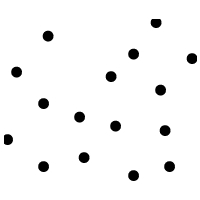
\includegraphics[width=40mm]{Figure_1}
\caption{A 'map' of 16 cities the salesman must travel to}
\label{overflow}
\end{figure}
Suppose the salesman has a map in front of him with 16 points he has to visit, as in Figure 1.1. If we let the salesman start at an arbitrary point, where should he travel from there? For example, if the salesman starts at the point in the bottom middle of the picture (see Figure 1.2), he has four candidates that all seem like equally good choices to travel to. 
\begin{figure}[ht!]
\centering
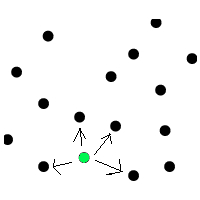
\includegraphics[width=40mm]{Figure_2.jpg}
\caption{If he starts at this spot, there are some 'good looking' choices}
\label{overflow}
\end{figure}
But perhaps one of those paths would lead to an unoptimized route down the line, so in fact the salesman cannot consider only the paths that 'look good' from where he is, but must exhaustively check every possible combination. Since he cannot return to a city he has previously visited, that means he will have $n!$ (in this case, $16! = 2.09 \cdot 10^{13}$) possible routes to choose between. 
\begin{figure}[ht!]
\centering
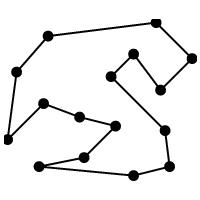
\includegraphics[width=40mm]{Figure_3}
\caption{The final, optimal solution}
\label{overflow}
\end{figure}

%
%
%
\section{Naive Recursive Approach}
As stated before, in a naive approach we'll have to exhaustively search through all $n!$ possible routes for the salesman to take. This approach would look something like the following:

%%%%%%
\subsection{Code Listing - Naive}
\lstset{escapechar=\@}
\lstset{tabsize=2}
 \begin{lstlisting}
 
 bestRoute = null
 shortestDistance = MAX_DOUBLE
 
@\emph{findOptimalRoute}@(currentRoute, citiesNotInRoute) {
	if (citiesNotInRoute is non-empty) {
		for (@$i = 1 \dots$@ citiesNotInRoute)
			tempCity = citiesNotInRoute.removeNextCity()
			newRoute = currentRoute.clone()
			newRoute.add(tempCity)
			
			findOptimalRoute(newRoute, citiesNotInRoute)
			citiesNotInRoute.remove(tempCity)
		}
	}
	else {
		if (currentRoute.distance < shortestDistance) {
			shortestDistance = currentRoute.distance
			bestRoute = currentRoute
		}
	}
}
	
\end{lstlisting}   
%%%%%
\subsection{Analysis of Naive Recursive Algorithm}

The basic idea of the code listed above is to do an exhaustive search; try every possible city as the 'start city,' then test ever possible route to each of the other cities. There is a small caveat that we will need to travel back to the start city from the final city to make it a cycle, but this is a small change and very trivial to implement. \\
\indent This algorithm has major inefficiencies. Let's say that our initial call was with a map containing $n$ cities, which took $\delta$ recursive calls to solve. Then to solve $\Delta =$ findOptimalRoute(null, $n+1$ cities) we can see that we will first have to put that city as the start city and then do $\delta$ calls to find the optimal route through the other $n$ cities. However, for each of the other n cities, when that city is the start city in the algorithm we will again have to do $\delta$ calls to solve the optimal route with that city as the start.\\ 
\indent This means that to go from $n$ to $n+1$ we will have to make $\Delta = (\delta + 1)\cdot \delta$ calls, or in other words $T(n) = n\cdot(n-1)$, which means this algorithm is $O(n!)$. Clearly this just will not do, as no experimentation is needed to show that the runtime quickly escales: 
\[
5! = 120 \dots 25! = 1.5 \cdot 10^{25} \dots 50! = 3 \cdot 10^{64} 
\]
However, the one positive part of this algorithm is that it does in fact generate the optimal solution every time, which is something that no other algorithm can claim.
%%%%%%%%

\section{Dynamic Programming Approach}

The Traveling Salesman problem is one of the most studied and talked about problems in computer science. I think it's kind of silly that I'm explaining it to you when there are many better resources out there, but I'll do my best to detail an efficient (though non-optimal) Dynamic Programming approach to the problem. \\
\indent In order to solve the Euclidean TSP in a more efficient way, we will break it up into two steps. First, we will generate a Minimum Spanning Tree from our cities. Next, we will do a Depth-First Search through the tree to generate our route. \\
\indent Minimum Spanning Trees are a subject of graph theory, and can be explained simply as a set of edges that connects all vertices in the graph (connectedness in the graph theory sense of the word- a $u-v$ path for all vertices $u, v \in V(G)$) such that the total edge distance is minimized. \\
\indent In Figure 3.1 we can see how the MST follows from a set of vertices.

\begin{figure}[ht!]
\centering
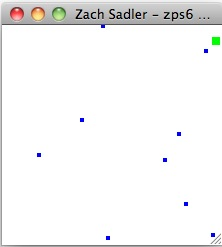
\includegraphics[width=40mm]{Figure_4}\,\,\,\,\,\,\,\,\,\,\,\,\,\,\,\,\,\,\,\,\,\,\,\,\,\,\,\,\,\,\,\,\,\,\,\,\,
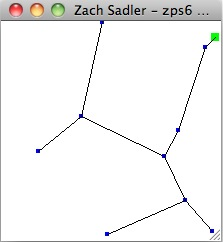
\includegraphics[width=40mm]{Figure_5}
\caption{A set of vertices and the MST that follows}
\label{overflow}
\end{figure}


%%%%%

\subsection{Code Listing 2 - Prim's Algorithm}
One simple algorithm that can find a MST of a graph is Prim's algorithm. Prim's algorithm will start with an arbitrary vertex and seek out new vertices to add to the unfinished MST by looking for the verex which is closest to the tree, adding it to the tree, and continuing until it has encompassed all vertices. Along the way it will keep track of the edges it has linked up, so that later we can read through the full MST. 
\begin{lstlisting}

@\emph{prim}@(vertices) {
	finishedVertices.add(vertices.get(arbitraryNumber))
	vertices.remove(arbitaryNumber)
	
	while (vertices is not empty) {
		vertexToAdd = null
		vertexToAddTo = null
		min = Double.MAX_DOUBLE
				
		for (@$v_i$@ in vertices) {
			for (@$v_j$@ in finishedVertices) {
				if (@$v_i$.distanceTo($v_j$)@ < min) {
					min = @$v_1$.distanceTo($v_j$)@
  					vertexToAdd = @$v_i$@
  					vertexToAddTo = @$v_j$@
				}
			}
		}
		
		finishedVertices.add(vertexToAdd)
		vertices.remove(vertexToAdd)
		edges.add(new Edge(vertexToAdd, vertexToAddTo)
	}
}
\end{lstlisting}

\subsection{Analysis of Dynamic Bottom-up Algorithm}

This version of Prim's Algorithm will take $O(n^2)$ calls, which is just fine for our purposes. Ther is no recursion, just a simple double for loop through a shrinking and an increasing set of vertices, contained within a while loop. Prim's algorithm sucessfully finds the MST (the Minimum of all the spanning trees).

\subsection{Code Listing 3 - Depth First Search}

Now that we have our MST, we can generate an actual route for the salesman to take. To do this we will begin at the start city (which was chosen arbitrarily before), and recursively explore all of its adjacent vertices, marking them as 'checked' as we go. If we encounter an unchecked vertex then we explore its adjacencies, otherwise we just return and add it to the finished route. The pseudo-code follows:
 
\begin{lstlisting}

void @\emph{solveTour}@(vertex) {
	marked[vertex] = true
	for (int w : getId(vertex).adjacentTo) {
		if (not marked[w]) {
			solveTour(w)
			tour.add(getId(w))
		}
	}		
}

route @\emph{putTogetherRoute}@() {
	route = new ArrayList<Edge>
	for (int i = 0; i + 1 < tour.size(); i++) {
		route.add(new Edge(tour.get(i), tour.get(i+1)))
	}
	route.add(new Edge(tour.get(tour.size() - 1), tour.get(0)))
	return route
}
\end{lstlisting}

\subsection{Analysis of Depth First Search}

While this algorithm seems suspsiciously simple, it really is as easy as it seems. We simply visit each node, and explore as deep into its adjacencies as we can recursively. Then we begin backtracing, and adding to an array of vertices that we will later construct the route from. To construct the route we simple add an edge between vertex $v_i$ and vertex $v_{i+1}$, and then connect the final vertex to the initial vertex. \\
\indent In the worst case this algorithm will still only provide an answer twice as bad as the optimal solution, and as I will show through testing this algorithm often produces a value 1.56* the MST length.
\begin{figure}[ht!]
\centering
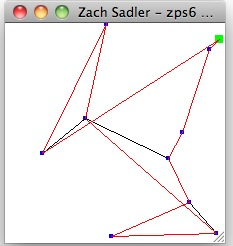
\includegraphics[width=40mm]{Figure_7}\,\,\,\,\,\,\,\,\,\,\,\,\,\,\,\,\,\,\,\,\,\,\,\,\,\,\,\,\,\,\,\,\,\,\,\,\,
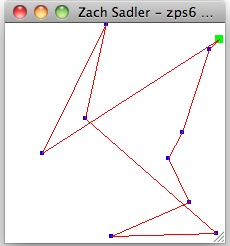
\includegraphics[width=40mm]{Figure_6}
\caption{The route overlayed on the MST (left) and standing alone (right)}
\label{overflow}
\end{figure}

%%%%%%%%%

\subsection{Further References}
As I mentioned earlier this is one of the most-studied problems in computer science and what I have explained so far in this paper hardly does the subject justice. For a more detailed look I suggest the following: \\
http://graphics.stanford.edu/courses/cs468-06-winter/Papers/arora-tsp.pdf \\
http://www.tsp.gatech.edu/index.html \\
http://www.ibm.com/developerworks/cloud/library/cl-optimizepythoncloud1/index.html 


\section{Results from Experimentation}
I wanted to test how close my program was to producing the optimal solution to the TSP. To do this I compared the length of my TSP route to the length of the MST given by Prim. I ran 5 trials each at a variety of number of cities, then averaged the result of how much larger my tour length was than the MST length. For example, at size $n = 10$ my results were 1.839, 1.660, 1.584, 1.541, and 1.717, so the AVG = 1.6682. The following table details my results:

\begin{table}[h]
\caption{Results from a Small Set of Experiments}
\centering
    \begin{tabular}{|l|l|l|l|l|l|l|}
        \hline
        Size of N    & 10 & 100 & 1000 & 2500    \\ \hline
        Trial 1    & 1.839 & 1.639 & 1.514 & 1.580    \\ \hline
        Trial 2    & 1.660 & 1.510 & 1.596 & 1.584    \\ \hline
        Trial 3    & 1.584 & 1.622 & 1.592 & 1.593    \\ \hline
        Trial 4    & 1.541 & 1.515 & 1.585 & 1.597    \\ \hline
        Trial 5    & 1.717 & 1.601 & 1.580 & 1.590    \\ \hline \hline
        Average & 1.6682 & 1.5774 & 1.5734 & 1.5888 \\
        \hline									
    \end{tabular}
\end{table}

Thus it seems like my program produces a route that is about 1.6 times the optimal solution. In comparison, the current best solution for the Euclidean TSP produces a route no worse than $(1 + 1/n)$ times the optimal route, according to \\
http://citeseer.ist.psu.edu/arora96polynomial.html

\section{Mandatory XKCD}
Because by now you're probably way more tired of reading these papers than we are of writing them, here's a relevant XKCD comic.
\begin{figure}[ht!]
\centering
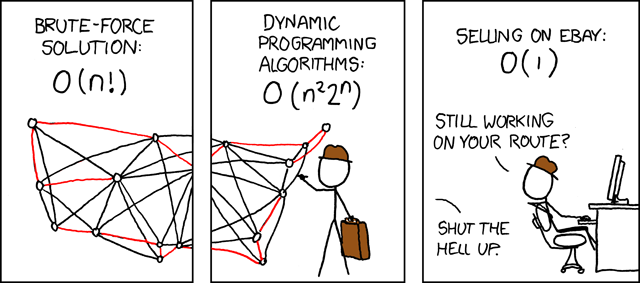
\includegraphics[width=122mm]{xkcd}
\label{overflow}
\end{figure}

\end{document}